\documentclass{beamer}
\usepackage[utf8]{inputenc}
\usepackage{pythonlisting}
\usepackage{graphicx}
\usepackage{multicol}
\newcommand{\cmark}{\ding{51}}%
\newcommand{\xmark}{\ding{55}}%

\useoutertheme{infolines}
\usetheme{Openwall}
\setbeamertemplate{navigation symbols}{}

\title{Inside Druva inSync}
\subtitle{Looking beyond marketing BS}
\author{Dhiru Kholia (dhiru@openwall.com)}
\date{19.06.2013}

\begin{document}

\frame{\titlepage}

\begin{frame}
	\frametitle{About Me}
	\begin{itemize}
		\item JtR, Ettercap and hashkill developer
		\item Metasploit and Nmap contributor
		\item \#openwall channel on Freenode
		\item @DhiruKholia on Twitter
	\end{itemize}
\end{frame}

\begin{frame}
	\frametitle{Agenda}
	\begin{itemize}
		\item About Druva inSync
		\item Authentication Issues
		\item Licensing Hack
		\item Remote code execution
		\item Misuse of SSL
		\item Bytecode Protection Issues
		\item Vendor Response
		\item Demo
	\end{itemize}
\end{frame}

\begin{frame}
	\frametitle{About inSync}
	\begin{itemize}
		\item Druva inSync is an on-premise and cloud-based
		backup software (Wikipedia)
		\item Druva provides enterprise laptop backup solutions that
		protect corporate users data with 10x faster backups and 90\% reduction
		in storage requirements (Twitter)
		\item The data is encrypted both during transit (256-bit SSL) and
		in the storage (256-bit AES).
	\end{itemize}
\end{frame}

\begin{frame}
	\frametitle{Popularity}
	\begin{itemize}
		\item 1,823 enterprises
		\item 1,324,587 endpoints
		\item 48 countries
		\item 98\% Customer Satisfaction Rate
		\item Customers include NASA, PwC, Deloitte, Amway, Xerox and McAfee among others
		\item Rated "excellent" by Gartner
		\item (June 2013 data)
	\end{itemize}
\end{frame}

\begin{frame}
	\frametitle{Security Claims}
	\begin{itemize}
		\item ``inSync Cloud offers the industry-best security.''
		\item SAS 70 Type II, PCI DSS Level 1, ISO 27001, ISAE 3000 Type I
		\item Industry-First Two-Factor Encryption. Even Druva can’t access your data.
		\item How do they do de-duplication? Does "dropship" like attack works?
	\end{itemize}
\end{frame}

\begin{frame}
	\frametitle{Authentication Database}
	\begin{itemize}
		\item "inSync Cloud offers the industry-best security"
		\item Password hashes are stored in a SQLite database file
		\item Uses single iteration of md5 to protect admin and user
		passwords. \textcolor{red}{hash = md5(id + password)}
		\item \textcolor{orange}{select id, name, emailid, password from administrator}
		\item Such hashes are crackable at high speeds using JtR
		or hashcat family of softwares. (4.2B c/s possible with
		oclHashcat-lite on AMD 7970)
		\item Ever heard about PBKDF2?
	\end{itemize}
\end{frame}

\begin{frame}
	\frametitle{MD5}
	\begin{center}
		
\includegraphics[scale=1]{meme-md5}
	\end{center}
\end{frame}

\begin{frame}
	\frametitle{inSync Licensing}
	\begin{itemize}
		\item Trial license expires after 30 days
		\item Enterprise license is limited to 500 users per
		server.
		\item Need to pay extra \$\$\$ for features like file
		sharing, DLP and analytics and these are
		"time-bombed".
	\end{itemize}
\end{frame}

\begin{frame}
	\frametitle{Hacking Licensing}
	\begin{center}
		
\includegraphics[scale=0.28]{meme-license}
	\end{center}
\end{frame}

\begin{frame}
	\frametitle{License Hack}
	\begin{itemize}
		\item It is easy to reverse-engineer and generate unlimited
		Enterprise licenses.
		\begin{center}
			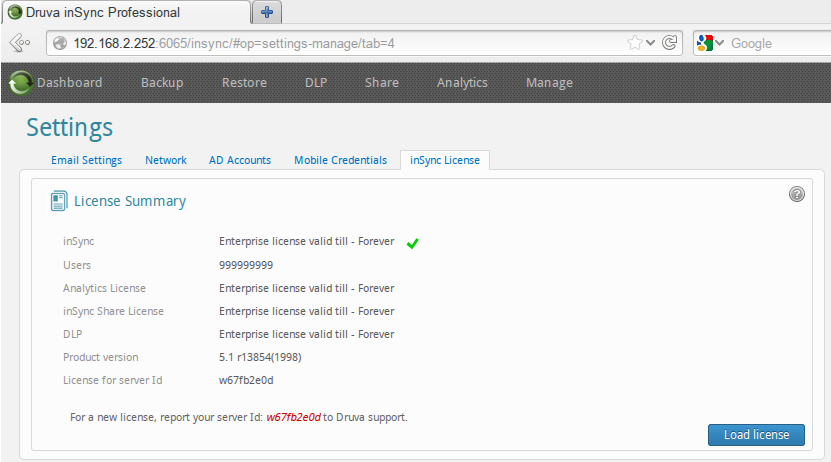
\includegraphics[scale=0.46]{license-hack}
		\end{center}
	\end{itemize}
\end{frame}

\begin{frame}[fragile]
	\frametitle{License Hack}
	\begin{itemize}
		\item inSync places md5 hash (of all fields) at the end of plain-text
		license string. Easy to manipulate and change numbers of users,
		expiration dates etc. Something like "a=b:md5(a=b)".
		\item inSync then "encrypts" this string with the following "encryption" function
	\end{itemize}

	\begin{center}
		\begin{python}
			def encrypt(in):
			return base64.b64encode(bz2.compress(in, 9))
		\end{python}
	\end{center}

	\begin{itemize}
		\item Such "encrypted" license strings are easy to "decrypt"
	\end{itemize}
\end{frame}

\begin{frame}
	\frametitle{Preventing License Hacks}
	\begin{center}
		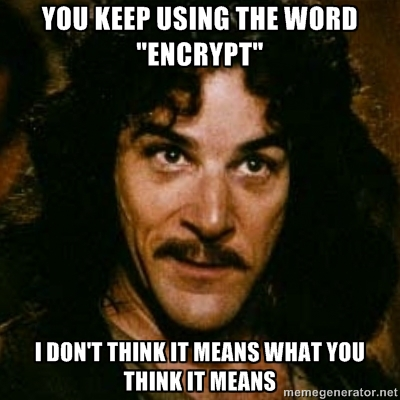
\includegraphics[scale=0.7]{meme-encrypt}
	\end{center}
\end{frame}

\begin{frame}
	\frametitle{Preventing License Hacks}
	\begin{itemize}
		\item Hard problem to solve.
		\item Even the industry "best" protection systems have been cracked (eventually)!
		\item Asymmetric cryptography can help? (WinRAR)
	\end{itemize}
\end{frame}

\begin{frame}
	\frametitle{SMTP configuration}
	\begin{itemize}
		\item It is mandatory to configure SMTP
		\item Same "encryption" function is used to "encrypt" SMTP password.
		\item Possible to do insidious social-engineering attacks if access
		to this SMTP account is gained.
	\end{itemize}
\end{frame}


\begin{frame}
	\frametitle{Better solution}
	\begin{itemize}
		\item Maybe try using CryptoAPI for slightly
		better protection.
	\end{itemize}
\end{frame}

\begin{frame}
	\frametitle{Arbitrary remote code execution}
	\begin{itemize}
		\item License files are in fact pickled strings.
		\item We can generate malicious license files!
		\item A successful social engineering attack on
		inSync administrator can lead to complete
		data loss!
	\end{itemize}
\end{frame}

\begin{frame}[fragile]
	\frametitle{pickle code execution}
	\begin{itemize}
		\item pickle is the standard mechanism for object serialization in Python
		\item By design, pickle allows code execution. It sure is convenient but isn't secure.
	\end{itemize}
	\begin{python}
		import pickle

		pickle.loads("cos\nsystem\n(S'ls ~'\ntR.")
	\end{python}
	\begin{itemize}
		\item This code runs "ls" command. Source: Nadia Alramli's Blog
		\item Google for "Sour Pickles Black Hat" for more information
	\end{itemize}
\end{frame}

\begin{frame}
	\frametitle{Arbitrary remote code execution}
	\begin{itemize}
		\item Never do "pickle.load(file\_handle)" when data
		source is not trusted and controlled.
		\item By design, pickle allows code execution. It
		sure is convenient but isn't secure.
		\item Writing your own custom plain-text format is
		trivial (or just use JSON).
	\end{itemize}
\end{frame}

\begin{frame}
	\frametitle{on-the-wire data protection claims}
	\begin{itemize}
		\item "inSync Cloud offers the industry-best security"
		\item "256-bit SSL encryption for data in transit"
		\item "Secure HTTPS and LDAPS protocols for
		access"
	\end{itemize}
\end{frame}

\begin{frame}
	\frametitle{Reality}
	\begin{center}
		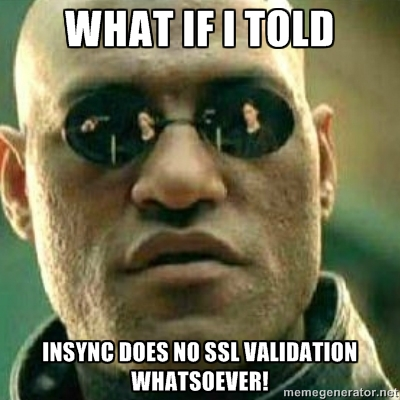
\includegraphics[scale=0.7]{meme-1}
	\end{center}
\end{frame}


\begin{frame}
	\frametitle{Reality}
	\begin{itemize}
		\item 256-bit SSL? Sure
		\item However, \textcolor{red}{No SSL certificate verification is done.}
		\item inSync client (installed on end devices) does NO verification of SSL certificates whatsoever. \#epicfail
		\item Hello MiTM attacks!
	\end{itemize}
\end{frame}

\begin{frame}
	\frametitle{MiTM code}
	\begin{itemize}
		\item https://github.com/kholia/ettercap/tree/inSync
		\item Allows to steal passwords or "hashes"
		\item Anyone of them can be used to steal (or wipe) all data!
	\end{itemize}
\end{frame}

\begin{frame}
	\frametitle{MiTM prevention}
	\begin{itemize}
		\item "256-bit SSL encryption" text is used for
		pure marketing purposes by Druva.
		\item 256-bit doesn’t do any good if you are not doing
		SSL certificate validation
		\item Deploy "real" certificates on inSync server for best
		results
		\item Publish (and verify) certificate fingerprint
	\end{itemize}
\end{frame}

\begin{frame}
	\frametitle{(lack of) Bytecode Protection}
	\begin{itemize}
		\item Druva uses py2exe (on Windows) to bundle and
		distribute inSync
		\item It is easy to reverse-engineer Druva inSync.
		\item unzip command + a Python decompiler (uncompyle2) are enough to obtain complete source-code of inSync.
	\end{itemize}
\end{frame}

\begin{frame}[fragile]
	\frametitle{Generic "unpacker"}
	\begin{python}
		import zipfile

		fileName = "inSync"

		ztype = zipfile.ZIP_DEFLATED

		f = zipfile.PyZipFile(fileName, "r", ztype)

		f.extractall("pyc_orig")
	\end{python}
\end{frame}

\begin{frame}
	\frametitle{Decompiling bytecode}
	\begin{itemize}
		\item https://github.com/Mysterie/uncompyle2
		\item As easy as doing "uncompyle2 -o hello.py hello.pyc"
		\item There is no protection whatsoever. Have fun ;)
	\end{itemize}
\end{frame}


\begin{frame}
	\frametitle{Bytecode Protection Techniques}
	\begin{itemize}
		\item Opcode obfuscation
		\item Bytecode encryption
		\item Booby-trapped customized python27.dll (like Dropbox) ;)
		\item Static linking of Python interpreter
	\end{itemize}
\end{frame}

\begin{frame}
	\frametitle{Vendor Response}
	\begin{block}{My Thoughts}
		Companies don't see it as a security problem;
		they see it as a PR problem" - Bruce Schneier on security issues.
	\end{block}
	\begin{itemize}
		\item Contacted vendor on 18th December 2012. They asked for
		      "details" which I sent promptly. No further contact.
		\item Contacted CEO and CTO on 2nd January 2013.
		\item Got vendor response on 27th March 2013. Druva is working
		      on fixing some of the problems.
	\end{itemize}
\end{frame}

\begin{frame}
	\frametitle{Twitter Encounter}
	\begin{center}
		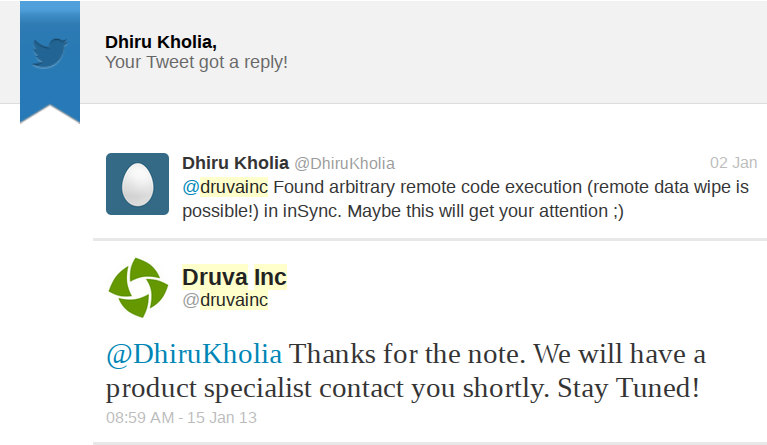
\includegraphics[scale=0.4]{twitter}
	\end{center}

	They deleted their own tweet for unknown reasons ;)

\end{frame}


\begin{frame}
	\frametitle{Don’t repeat mistakes @druvainc}
	\begin{itemize}
		\item LinkedIn leak (6.5 million SHA1 hashes, over 90\% of them got cracked!)
		\item Best not to invent your own crazy schemes
		\item Read up on PBKDF2
		\item Stop misusing / using pickle
		\item Compression is not "encryption" (and hashing is not encryption)
	\end{itemize}
\end{frame}

\begin{frame}
	\frametitle{Future Work}
	\begin{itemize}
		\item Obtain trial to their cloud version of inSync and
		break it. Any help is welcome!
		\item Understand inSync’s key derivation process.
		Most likely it will be single iteration of MD5 \#lol
		\item Reverse-engineer custom storage "blob" format used by inSync
		\item Can we run from decompiled "sources"?
		\item What about releasing an open-source Druva inSync client? ;)
	\end{itemize}
\end{frame}

\begin{frame}
	\frametitle{Questions?}
\end{frame}

\begin{frame}
	\frametitle{DEMO!}
	\begin{itemize}
		\item http://www.druva.com/insync-enterprise-releases
		\item Extracting bytecode
		\item De-compiling bytecode
	\end{itemize}
\end{frame}

\begin{frame}
	\frametitle{Thanks!}
	\begin{center}
		
\includegraphics[scale=0.35]{thanks}
	\end{center}
\end{frame}

\end{document}
